\documentclass[a4paper]{report}
\usepackage[utf8]{inputenc}
\usepackage[portuguese]{babel}
\usepackage{hyperref}
\usepackage{a4wide}
\hypersetup{pdftitle={MDIO - Trabalho 2},
pdfauthor={João Teixeira, José Ferreira, Miguel Solino},
colorlinks=true,
urlcolor=blue,
linkcolor=black}
\usepackage{subcaption}
\usepackage[cache=false]{minted}
\usepackage{listings}
\usepackage{booktabs}
\usepackage{multirow}
\usepackage{appendix}
\usepackage{tikz}
\usepackage{authblk}
\usepackage{bashful}
\usepackage{verbatim}
\usepackage{amsmath}
\usetikzlibrary{positioning,automata,decorations.markings}
\AfterEndEnvironment{figure}{\noindent\ignorespaces}

\begin{document}

\title{MDIO - Trabalho 2\\ 
\large Grupo Nº 3}
\author{João Teixeira (A85504) \and José Ferreira (A83683) \and Miguel Solino (A86435)}
\date{\today}

\begin{center}
    \begin{minipage}{0.75\linewidth}
        \centering
        
\includegraphics[width=0.4\textwidth]{images/eng.jpeg}\par\vspace{1cm}
        \vspace{1.5cm}
        \href{https://www.uminho.pt/PT}
        {\color{black}{\scshape\LARGE Universidade do Minho}} \par
        \vspace{1cm}
        \href{https://www.di.uminho.pt/}
        {\color{black}{\scshape\Large Departamento de Informática}} \par
        \vspace{1.5cm}
        \maketitle
    \end{minipage}
\end{center}

\tableofcontents

\pagebreak

\chapter{Introdução}
Um dos problemas \textit{NP-Completo} mais conhecido é o \textit{Travelling
Salesman Problem}. \\
Neste problema, um vendedor tem um conjunto de cidades que pretende visitar. As
estradas entre essas cidades e e a distancia destas também são conhecidas. O
objetivo deste problema é calcular o caminho mais curto que visite todas as
cidades.\\
Quando transferido para um grafo orientado, este problema resume-se
encontrar o caminho mais curto que visite todos os nodos do grafo.\\
Um problema derivado do \textit{Travelling Salesman Problem} é o \textit{Chinese
Postman Problem}.\\
Neste, um carteiro pretende entregar todas as cartas que tem, e para isso tem de
passar em todas as ruas pelo menos uma vez. Com o objetivo de percorrer a menor
distância possível.\\
Quando transferido para um problema de grafos, a única diferença entre este
problema e o problema do caixeiro viajante é que se pretende obter o caminho
mais curto que visite todas as arestas de um grafo orientado. \\
O objetivo deste projeto é resolver este problema utilizando \textit{RELAX4}

\chapter{Parte I}
\section{Problema}
Observando os números de inscrição dos membros do grupo, constatamos
que o maior pertencia ao aluno Miguel Solino (86435).
Fazendo \textit{pattern matching} para o padrão ABCDE e seguindo as
regras definidas no enunciado, concluímos que a orientação das ruas é:

\begin{enumerate}
    \item A é igual a 8;
    \item B é igual a 6, logo é par, e por isso aponta para baixo;
    \item C é igual a 4, logo é par, e por isso aponta para a direita;
    \item D é igual a 3, logo é ímpar, e por isso aponta para cima;
    \item E é igual a 5, logo é ímpar, e por isso aponta para a 
        esquerda;
\end{enumerate}
Assim, conclui-se que o problema a resolver é representado pela
seguinte imagem:

\begin{figure}[H]
    \begin{center}
        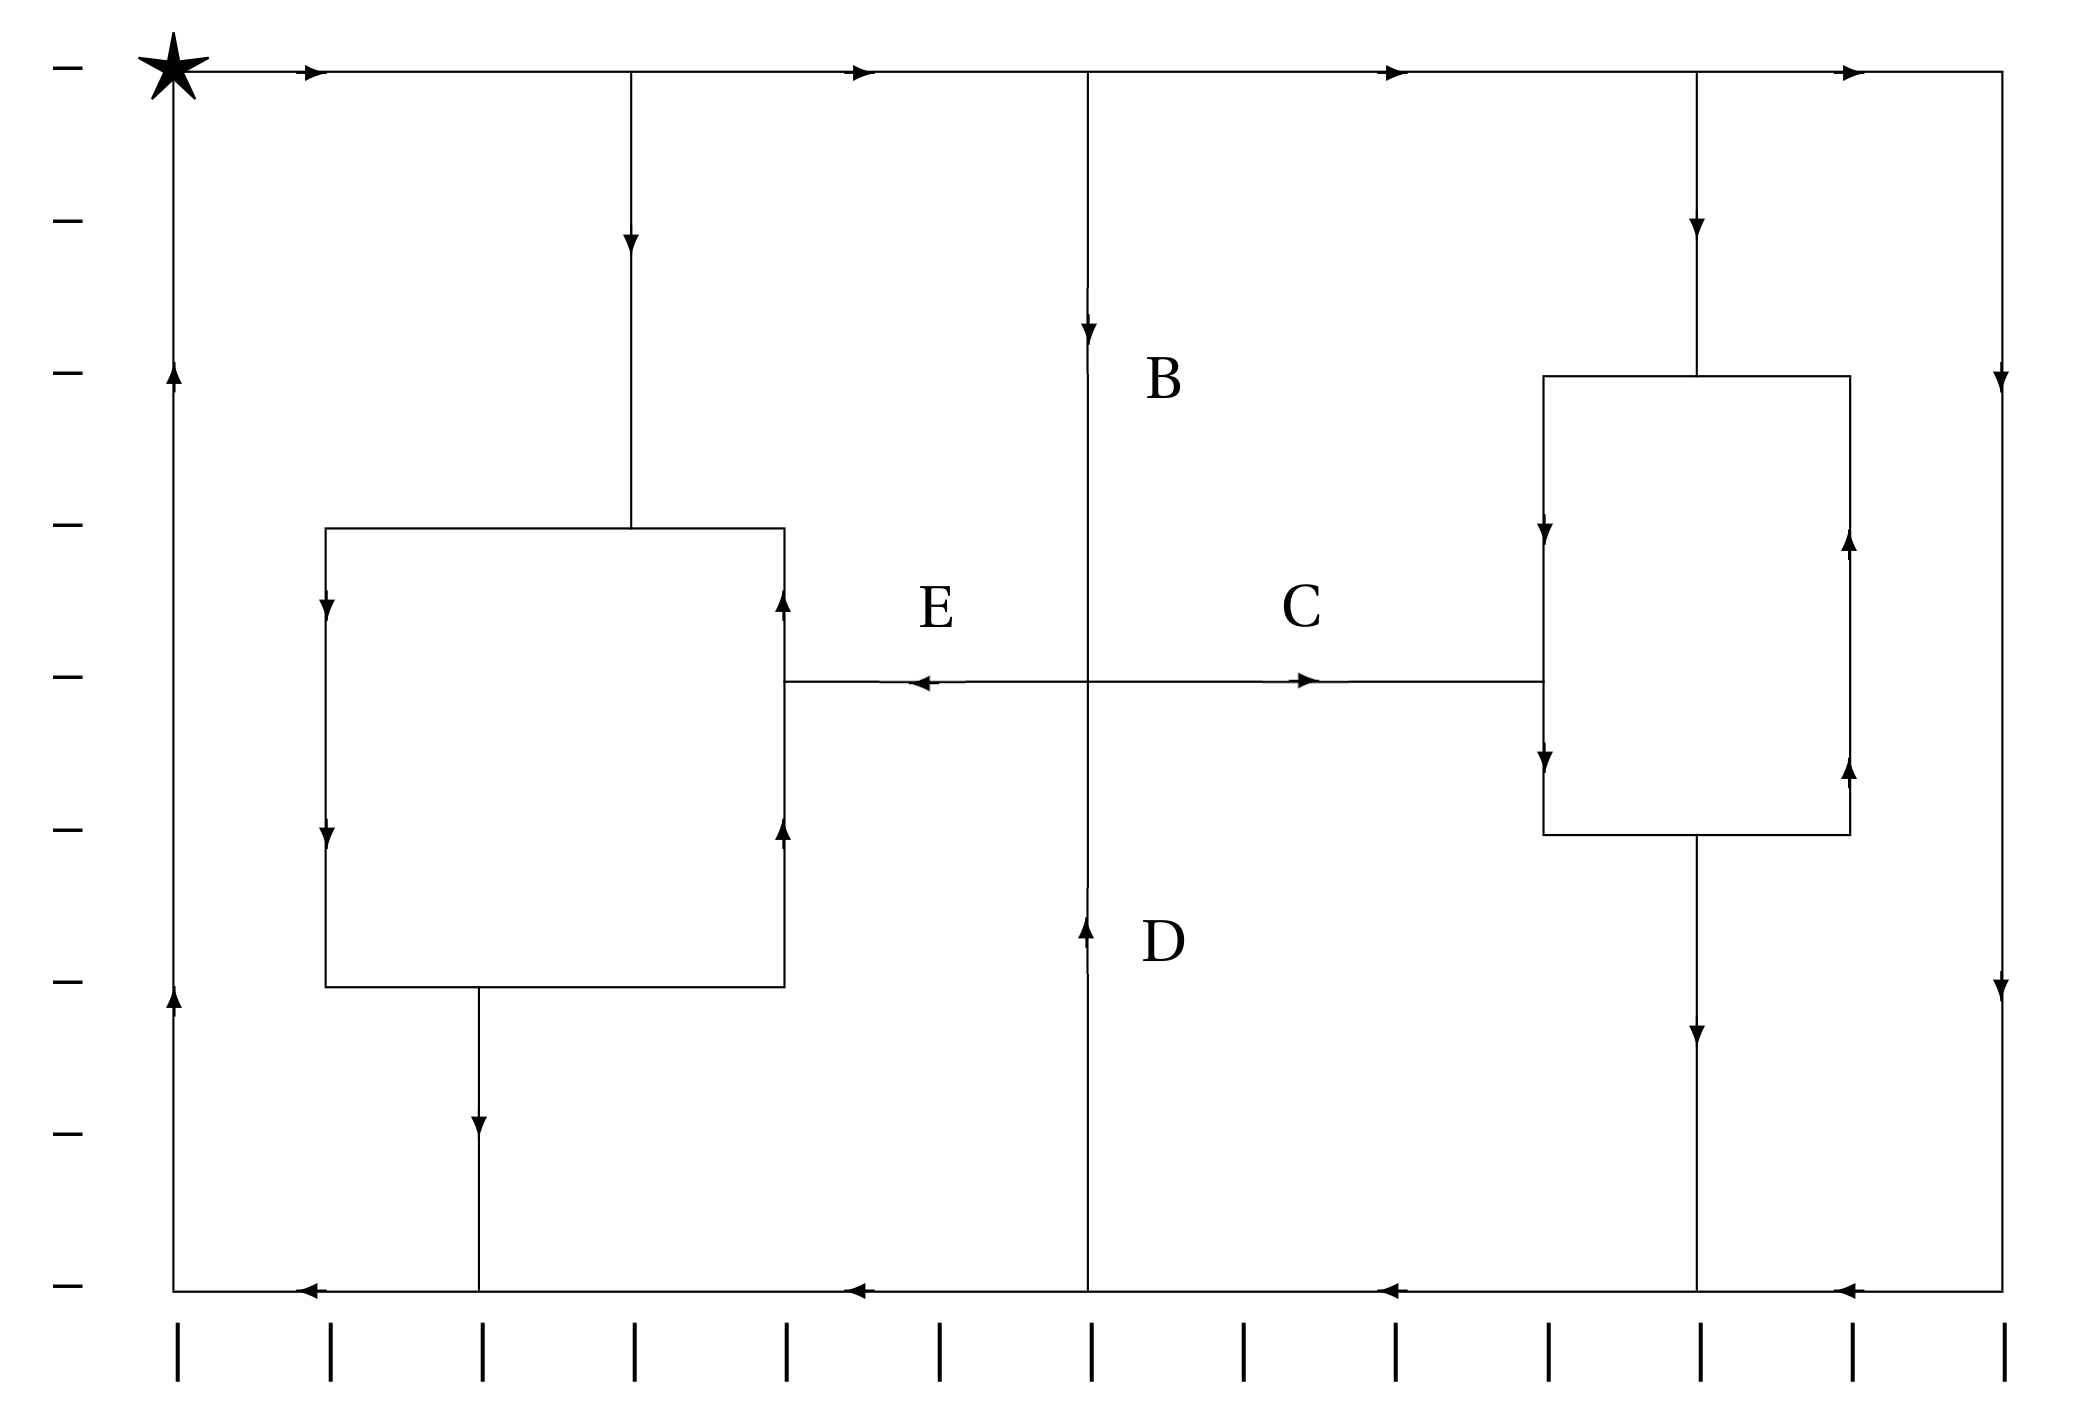
\includegraphics[width=0.9\textwidth]{images/desafio.png}\par
        \caption{representação do problema}
        \label{fig:problem}
    \end{center}
\end{figure}
Após obter esta imagem decidimos nomear cada vértice do problema com
uma letra maiúscula. Assim, o aspeto do desafio final utilizada é:

\begin{figure}[H]
    \begin{center}
        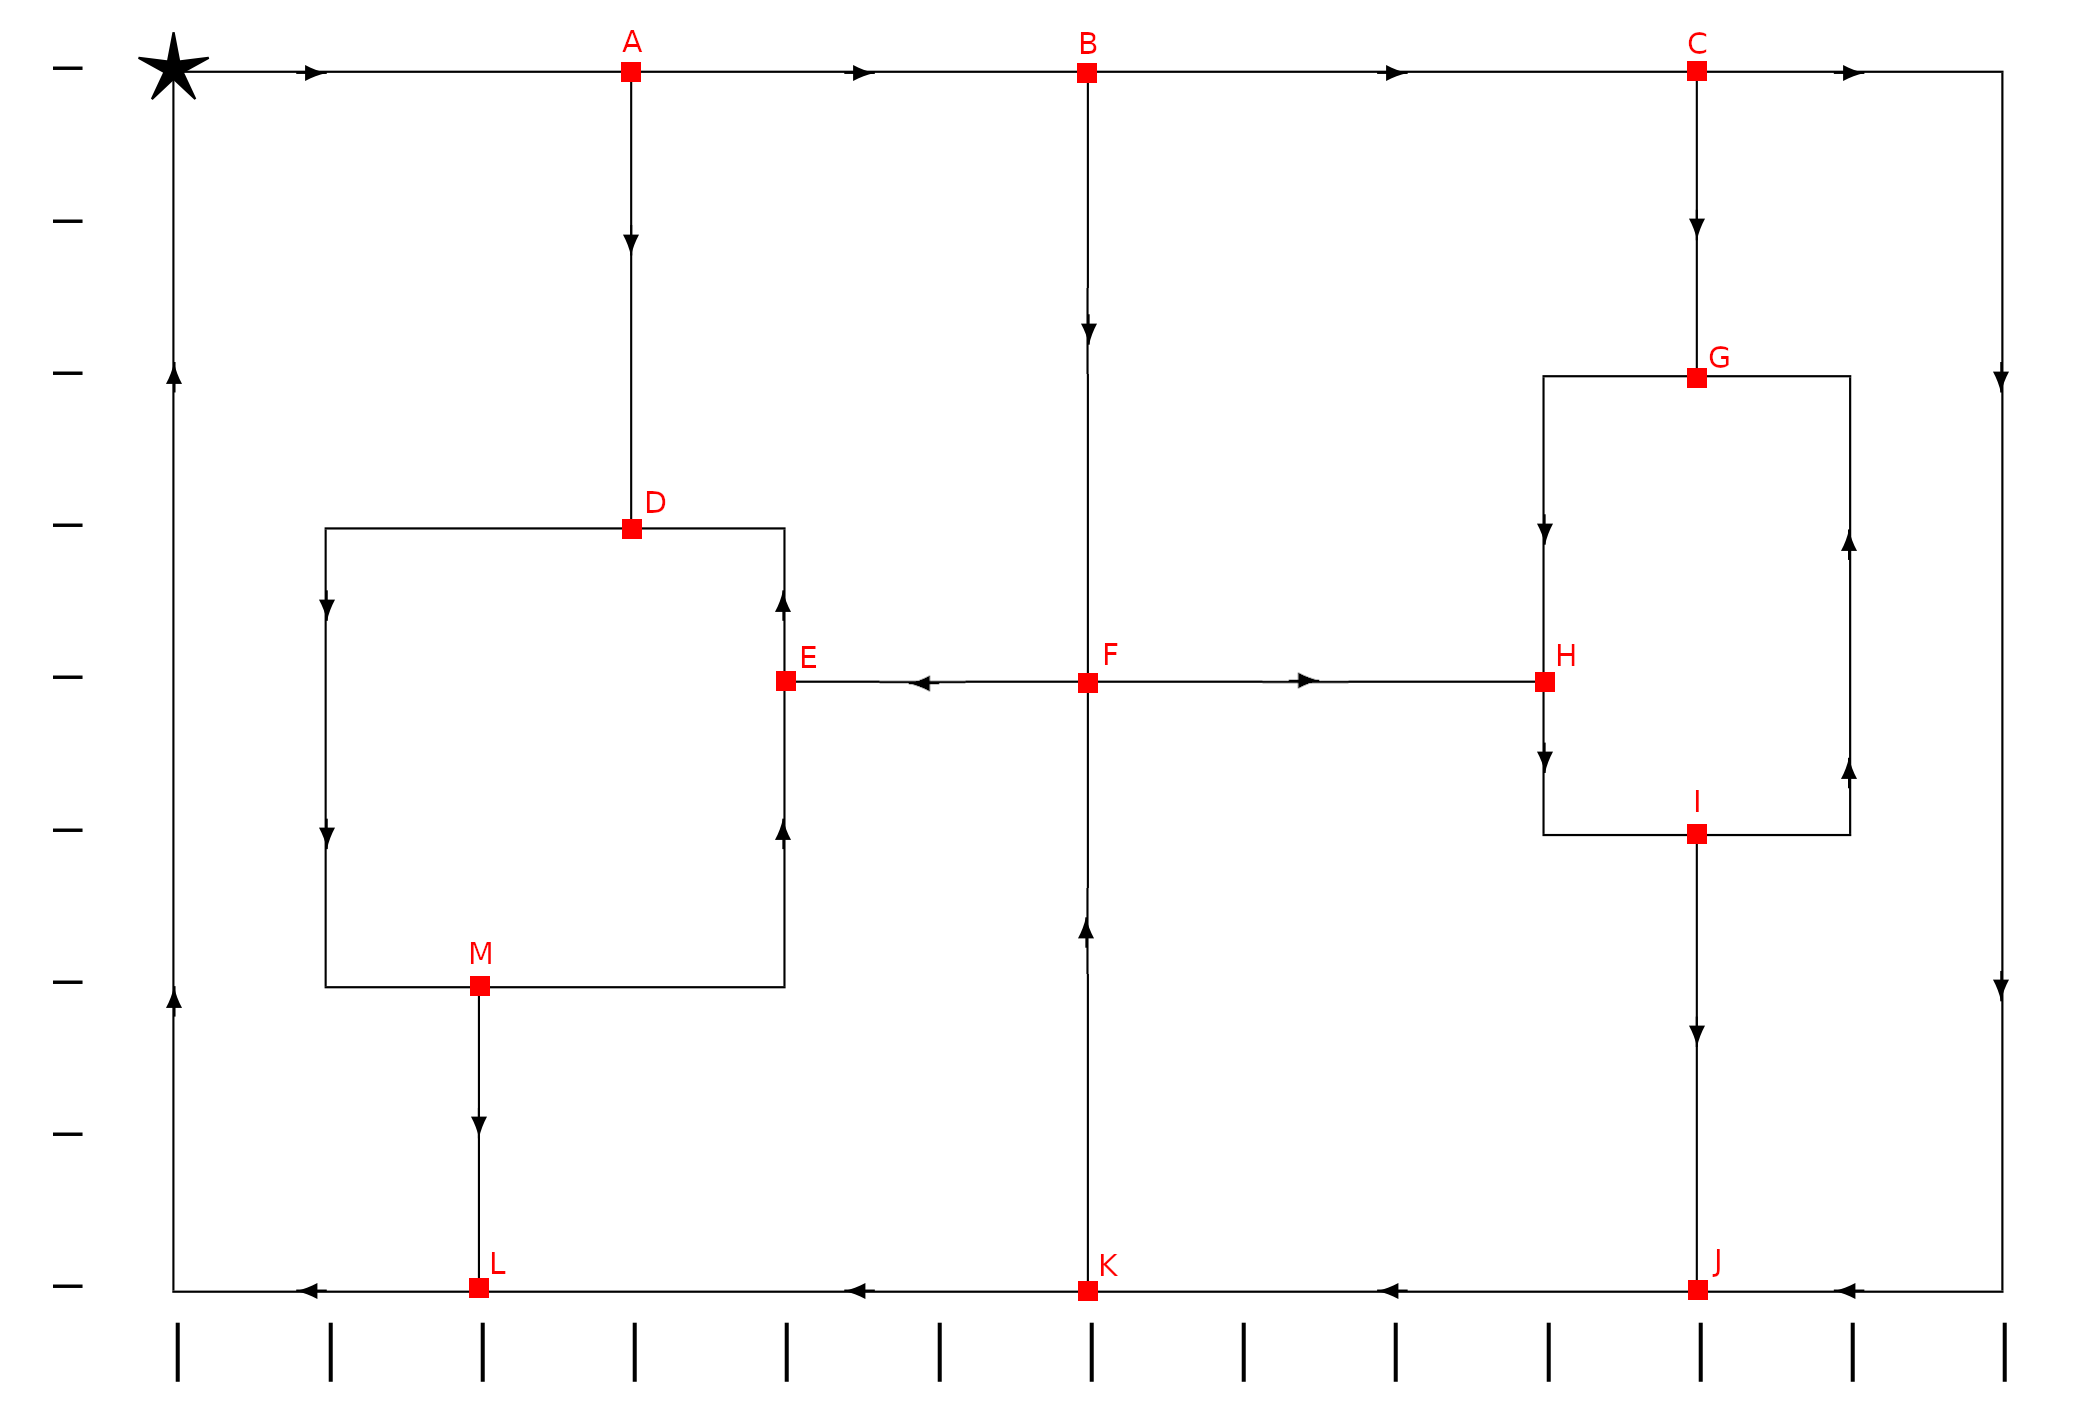
\includegraphics[width=0.9\textwidth]{images/desafioLetras.png}\par
        \caption{vértices nomeados}
        \label{fig:named}
    \end{center}
\end{figure}

\pagebreak
\section{Formulação do Problema}
Para esta primeira parte, o problema apresentado deve ser formulado como um
problema de transporte numa rede geral \textit{G=(V, A)}.

\subsection{Arestas}
A variável de decisão \textit{xij} representa o número de vezes que o arco (i,
j) foi percorrido.\\
Visto que o objetivo deste problema é que cada aresta seja visitada pelo menos
uma vez, é necessária a existencia de um bloco de condições que indiquem que
\textit{xij >= 1}.\\
No entanto, o \textit{software} de resolução de problemas em rede normalmente
apenas suporta arcos com um limite superior. Assim, aplica-se a mudança de
variável \textit{yij = xij - lij} em que \textit{lij} é o limite inferior de
fluxo no arco (i, j).\\
Aplicando esta mudança de variável à condição acima descrita obtemos que
\textit{xij >= 1} é equivalente a \textit{yij >= 0}.

\subsection{Nodos}
Para cada nodo no mapa, a soma de todas as vezes que se entra neste
tem de ser igual à soma de todas as vezes que se sai.\\
Assim, por exemplo, para o nodo A, o número de vezes que a aresta
\textit{xla} é percorrida tem de ser igual ao número de vezes que
as arestas \textit{xad} e \textit{xab} são percorridas.
Por exemplo, de forma a criar uma restrição para o nodo A, esta pode ser
formulada como:\\
\begin{multline}
- xla + xad + xab = 0 \\
\end{multline}
Aplicando a mudança de variável:
\begin{multline}
- (yla + 1) + (yad +1) + (yab +1) = 0 \\
\end{multline}
que pode ser simplificado para:
\begin{multline}
- yla + yad + yab = -1\\
\end{multline}

\pagebreak
\section{Modelo de Programação Linear alterado}
\verbatiminput{solution.lp}

\pagebreak
\section{Rede do Problema de Transporte}
De forma a que o input gerado para o \textit{RELAX4} seja válido é necessário
converter o nome dos nodos para números. Assim, o método utilizado é atribuir
como número a cada nodo o valor da posição da letra no alfabeto.


\subsection{Valores de Oferta}
\begin{itemize}
    \item Nodo D : 1
    \item Nodo E : 1
    \item Nodo G : 1
    \item Nodo H : 1
    \item Nodo J : 1
    \item Nodo L : 1
\end{itemize}

\subsection{Valores de Procura}
\begin{itemize}
    \item Nodo A : -1
    \item Nodo B : -1
    \item Nodo C : -1
    \item Nodo I : -1
    \item Nodo K : -1
    \item Nodo M : -1
\end{itemize}

\pagebreak
\section{Texto de Input}
\label{input}
\verbatiminput{RELAX4.INP}

\pagebreak
\section{Texto de Output}
\label{input}
\verbatiminput{RELAX4.OUT}

\pagebreak
\section{Interpretação do resultado}
\label{solution}
O valor obtido com o recurso ao \textit{relax4} é 87 (primeira linha do texto de
output). Uma vez que foi realizada uma mudança de variável, todas as arestas
foram visitadas n+1 vez do que a que é indicada na solução. Logo, para obter o
custo real do percurso obtido, é necessário somar ao valor obtido a soma de
todos os custos das arestas do grafo.\\
Assim, o custo do percurso obtido é igual a 87 + 85, que é igual a 172.\\
Visto que a solução ótima é um circuito fechado, independentemente do ponto
que se considere como o ponto inicial, este será sempre o mesmo. \\
Assim, de forma a facilitar a interpretação dos resultados consideramos como
ponto inicial o ponto A. Esta decisão em nada altera o problema.\\
A fim de facilitar a visualização dos resultados obtidos decidimos criar uma
imagem \ref{fig:visited} que indica para cada aresta o número de vezes que esta
foi visitada.

\begin{figure}[H]
    \begin{center}
        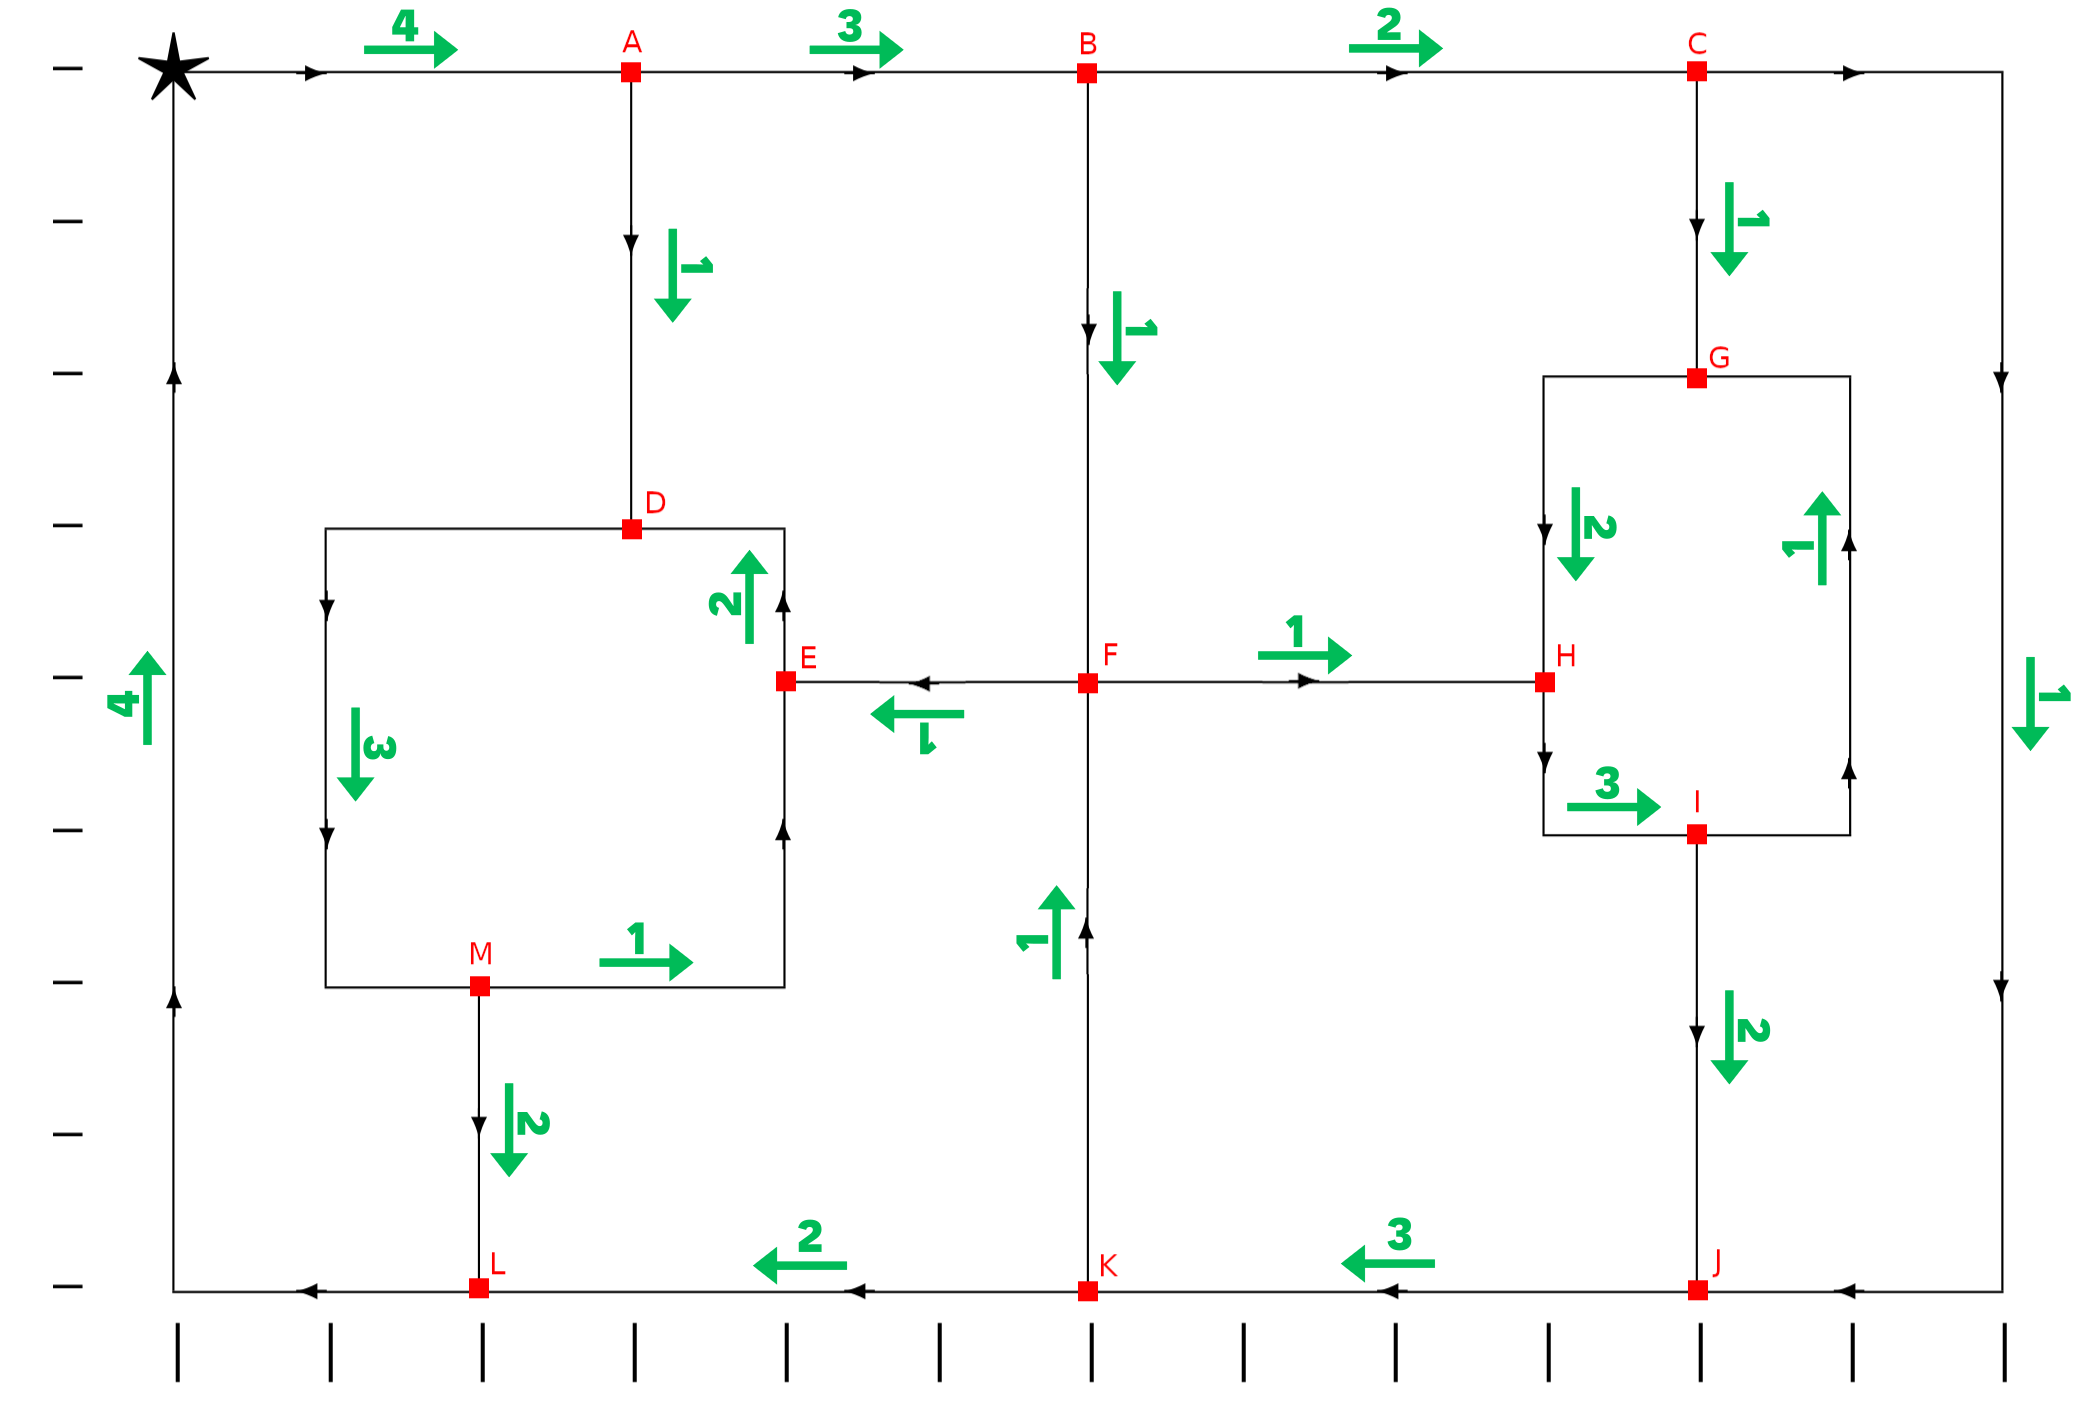
\includegraphics[width=0.8\textwidth]{images/desafioVisited.png}\par
        \caption{representação da solução}
        \label{fig:visited}
    \end{center}
\end{figure}
Na nossa solução (capitulo \ref{output}) a variável \textit{yla} é igual a 3, o
que quer dizer que esta aresta foi percorrida 4 vezes e na ultima vez todos os
outros tem de ter sido no mínimo percorridos uma vez.\\
Sabendo isto desenvolvemos a imagem \ref{fig:path} que contém o caminho ótimo
calculado. Este, está dividido em quatro percursos distintos que começam e
acabam em A.\\
Um dos problemas encontrados no cálculo destes caminhos é que uma aresta ter
sido visitada uma vez durante o percurso não implica que não volte a ser
visitada nesse mesmo percurso.

\begin{figure}[H]
    \begin{center}
        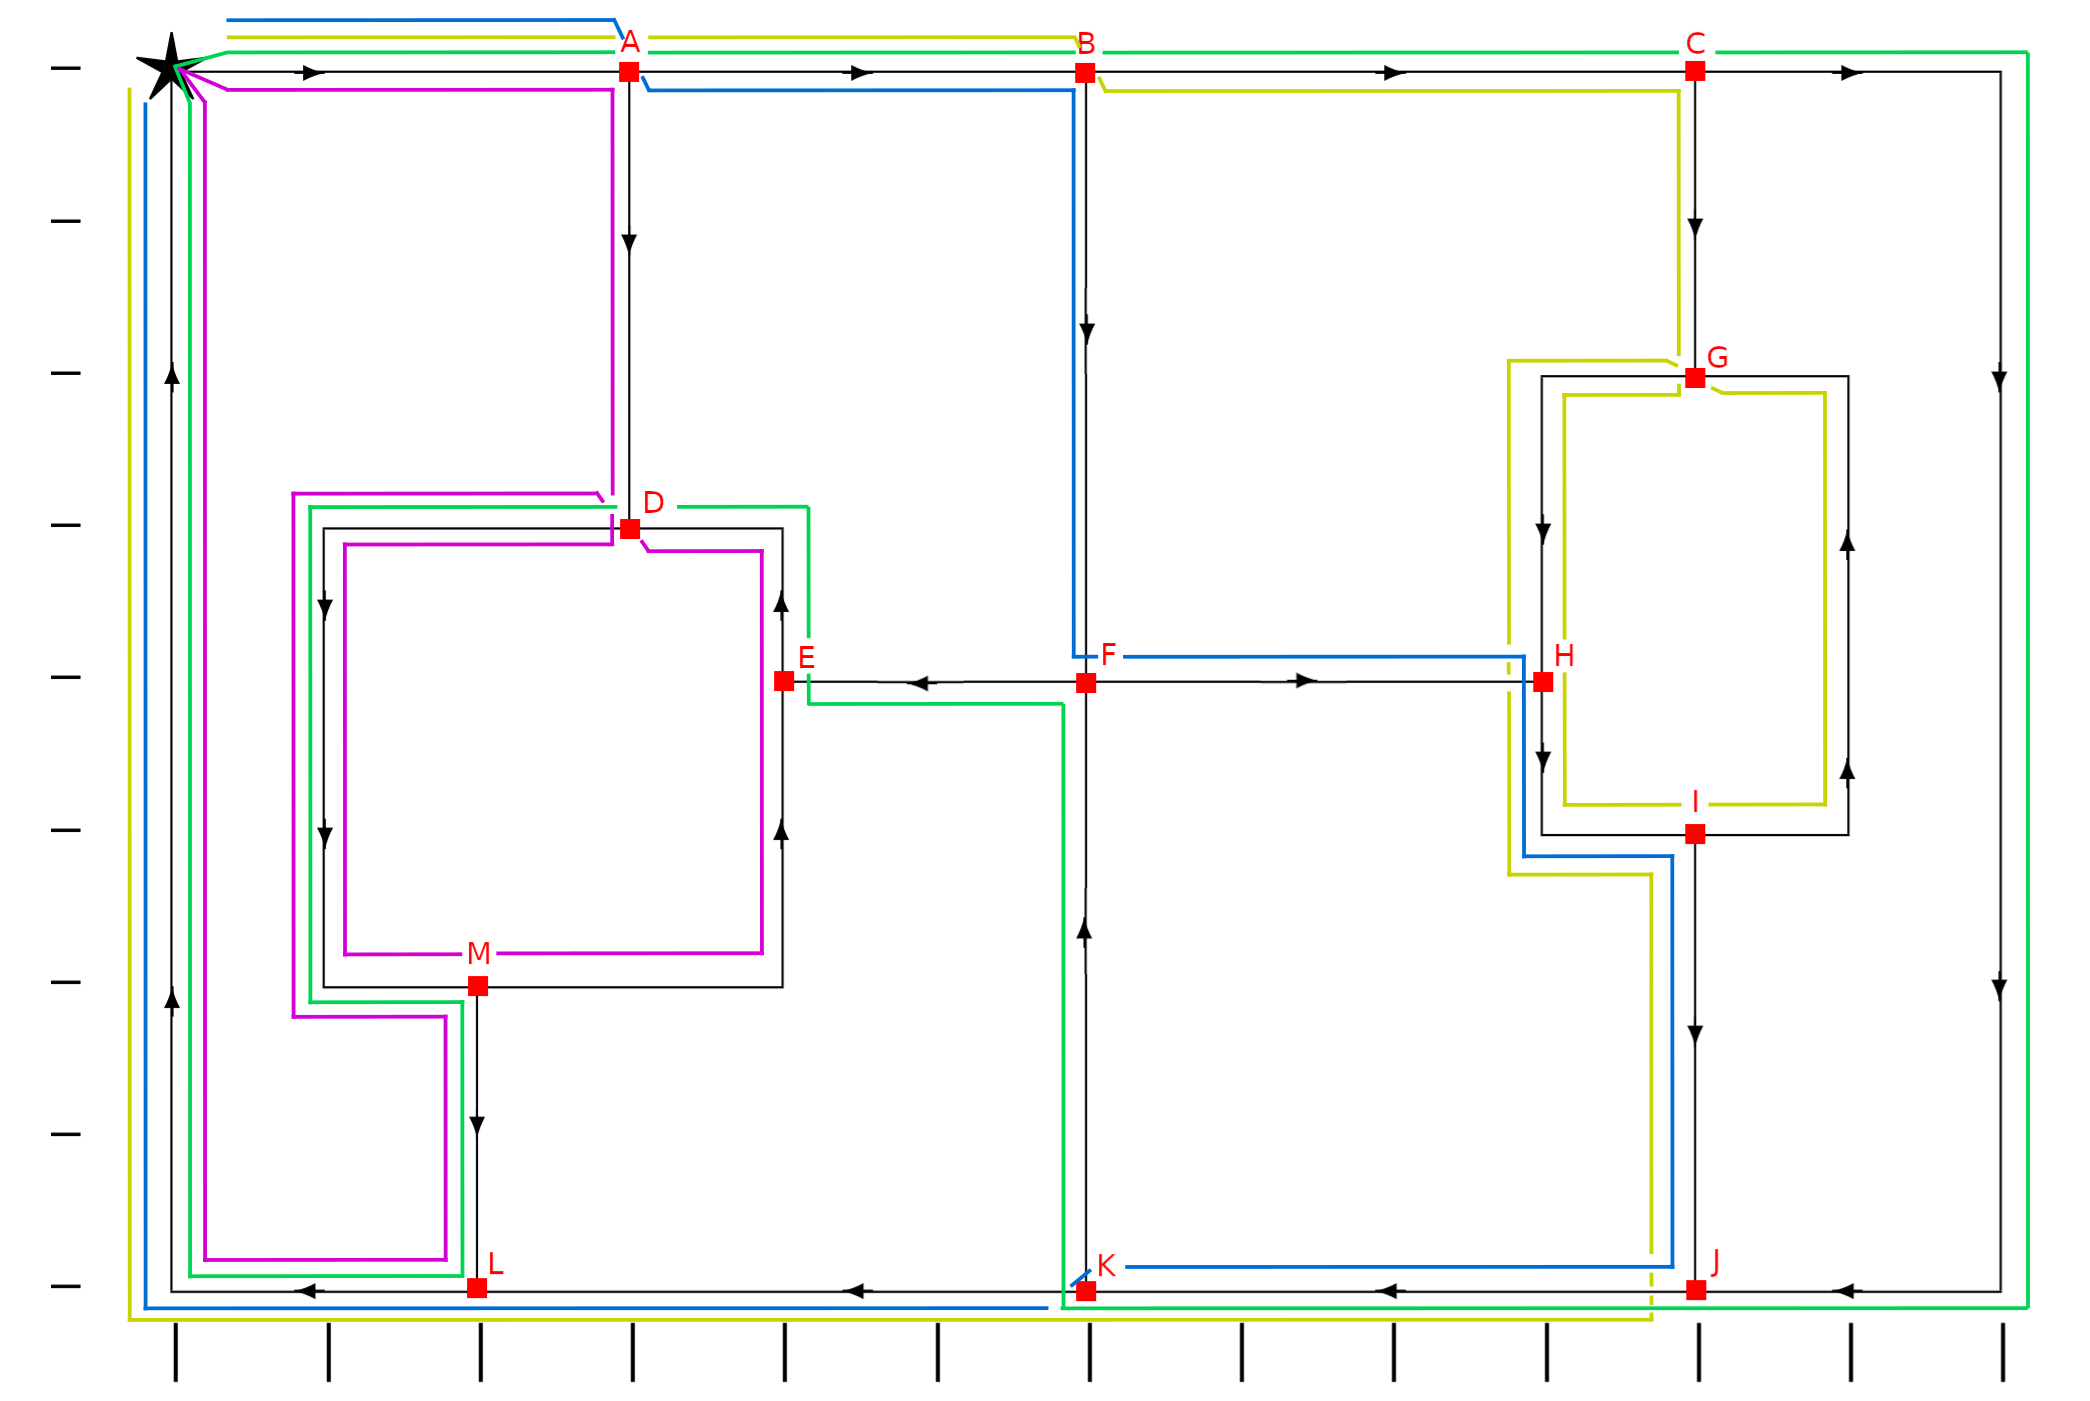
\includegraphics[width=0.9\textwidth]{images/desafioSolucao.png}\par
        \caption{representação do caminho}
        \label{fig:path}
    \end{center}
\end{figure}
A fim de facilitar a interpretação da imagem, elaboramos uma legenda para cada
um dos caminhos tomados:

\begin{enumerate}
    \item Verde: \\
    AB → BC → CJ → JK → KF → FE → ED → DM → ML → LA
    \item Amarelo: \\
    AB → BC → CG → GH → HI  → IG → GH → HI → IJ → JK  → KL  → LA
    \item Azul: \\
    AB → BF → FH→ HI  → IJ → JK  → KL  → LA
    \item Rosa: \\
    AD → DM → ME → ED  → DM → ML → LA
\end{enumerate}
Visto que estes 4 segmentos da solução ótima começam e acabam no nodo A podem
ser organizados por qualquer ordem que irá criar um percurso válido e sempre com
o mesmo custo. Assim, qualquer combinação destes 4 percurso produz uma solução
ótima válida para o problema apresentado.\\
De forma a apresentar uma solução concreta, escolhemos o percurso que consiste
em percorrer os segmentos da solução ótima pela ordem Verde → Amarelo → Azul →
Rosa. Este corresponde ao percurso:\\
AB → BC → CJ → JK → KF → FE → ED → DM → ML → LA →
AB → BC → CG → GH → HI  → IG → GH → HI → IJ → JK  → KL  → LA →
AB → BF → FH→ HI  → IJ → JK  → KL  → LA →
AD → DM → ME → ED  → DM → ML → LA

\pagebreak
\section{Validação do modelo}
\subsection{Tipo de variáveis}
As variáveis têm de ser todas do tipo inteiro pois representam o número
de vezes que essa aresta é atravessada. De facto, após analisar os resultados
obtidos, todos os resultados são valores inteiros.\\
Visto que é necessário que cada aresta seja visitada pelo menos uma
vez, todas as variáveis têm de ter um valor maior ou igual a zero, o
que de facto se verifica.

\subsection{Função objetivo}
O resultado da função objetivo utilizada no modelo quando o valor
das variáveis é manualmente substituindo pela solução ótima tem de 
coincidir com o resultado obtido.
Assim:

\begin{multline}
13\times yla + 3\times yab + 4\times ybc + 12\times ycj + 4\times
yjk + 4\times ykl + 4\times ykf + 2\times yfe + 2\times yed \\ + 6\times ydm +
2\times yml + 3\times yad + 4\times ybf + 3\times yfh + 2\times ycg +
3\times ygh + 2\times yhi + 3\times yij + 5\times yig + 4\times yme + 85
\end{multline}
E substituindo os valores das variáveis de decisão:
\begin{multline}
13\times 4 + 3\times 3 + 4\times 2 + 12\times 1 + 4\times
3 + 4\times 2 + 4\times 1 + 1 + 2\times 2 + 6\times 3 +
2\times 2 + 3\times 1 \\ + 4\times 1 + 3\times 1 + 2\times 1 +
3\times 2 + 2\times 3 + 3\times 2 + 5\times 1 + 4\times 1 + 85
= 172
\end{multline}

\subsection{Restrições}
\begin{multline}
A: - yla + yad + yab = -1
\Rightarrow - 3 + 0 + 2 = -1 
\Rightarrow -1 = -1
\end{multline}

\begin{multline}
B: - yab + ybf + ybc = -1
\Rightarrow - 2 + 0 + 1 = -1
\Rightarrow -1 = -1
\end{multline}

\begin{multline}
C: - ybc + ycg + ycj = -1
\Rightarrow - 1 + 0 + 0 = -1
\Rightarrow -1 = -1
\end{multline}

\begin{multline}
D: - yad - yed + ydm = 1
\Rightarrow - 0 - 1 + 2 = 1
\Rightarrow 1 = 1
\end{multline}

\begin{multline}
E: - yfe - yme + yed = 1
\Rightarrow - 0 - 0 + 1 = 1
\Rightarrow 1 = 1
\end{multline}

\begin{multline}
F: - ybf - ykf + yfe + yfh = 0
\Rightarrow - 0 - 0 + 0 + 0 = 0
\Rightarrow 0 = 0
\end{multline}

\begin{multline}
G: - ycg - yig + ygh = 1
\Rightarrow - 0 - 0 + 1 = 1
\Rightarrow 1 = 1
\end{multline}

\begin{multline}
H: - ygh - yfh + yhi = 1
\Rightarrow - 1 - 0 + 2 = 1
\Rightarrow 1 = 1
\end{multline}

\begin{multline}
I: - yhi + yig + yij = -1
\Rightarrow - 2 + 0 + 1 = -1
\Rightarrow -1 = -1
\end{multline}

\begin{multline}
J: - yij - ycj + yjk = 1
\Rightarrow - 1 - 0 + 2 = 1
\Rightarrow 1 = 1
\end{multline}

\begin{multline}
K: - yjk + ykf + ykl = -1
\Rightarrow - 2 + 0 + 1 = -1
\Rightarrow -1 = -1
\end{multline}

\begin{multline}
L: - yml - ykl + yla = 1
\Rightarrow - 1 - 1 + 3 = 1
\Rightarrow 1 = 1
\end{multline}

\begin{multline}
M: - ydm + yml + yme = -1
\Rightarrow - 2 + 1 + 0 = -1
\Rightarrow -1 = -1
\end{multline}


\chapter{Parte II}



\chapter{Conclusão}
Concluindo, com este trabalho implementamos uma solução para o problema do
Carteiro Chinês utilizando programação linear.\\
A solução ótima obtida tem uma distância total de 172 centímetros e um dos
percursos obtidos é (Capitulo \ref{solution}):\\
AB → BC → CJ → JK → KF → FE → ED → DM → ML → LA →
AB → BC → CG → GH → HI  → IG → GH → HI → IJ → JK  → KL  → LA →
AB → BF → FH→ HI  → IJ → JK  → KL  → LA →
AD → DM → ME → ED  → DM → ML → LA\\

\end{document}
